\documentclass[tikz]{standalone}
\begin{document}
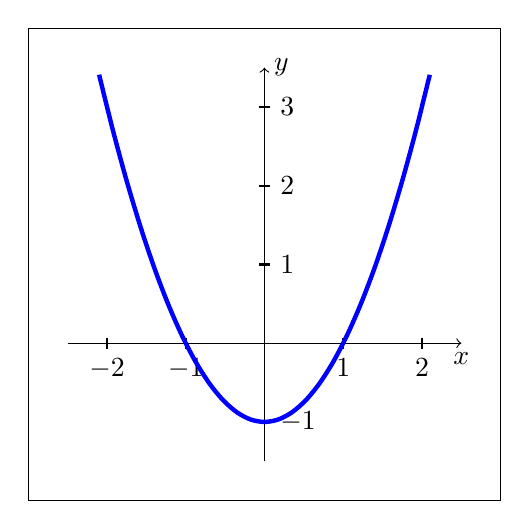
\begin{tikzpicture}[scale=1.0]

\draw[black,fill=white] (-3,-2) rectangle (3,4);
%\draw[very thin,color=lightgray,step=0.5] (-3.4,-4.9) grid (3.4,0.9);
%\draw[very thin,color=gray,step=2] (-3.5,-5) grid (3.5,1);

\draw[->] (-2.5,0) -- (2.5,0) node[below] {$x$};
\draw[->] (0,-1.5) -- (0,3.5) node[right] {$y$};
       
%s\node[right] at (0.9, -0.5){$y = x^2-4$};

% tick marks
\foreach \x in {-2,-1,1,2} 
	\draw [thick] (\x cm,2pt) -- (\x cm,-2pt) node[below] {$\x$};
\foreach \y in {-1,1,2,3} 
	\draw [thick] (-2pt,\y cm) -- (2pt,\y cm) node[right] {$\y$};


\draw[domain=-2.1:2.1,smooth,variable=\x,blue,ultra thick] plot ({\x},{\x*\x- 1});

\end{tikzpicture}
\end{document}

\noindent The domain of $f$ consists of all the different $x$-coordinates of points on the graph of $f$, which is $(-\infty,\infty)$.  The range of $f$ consists of all the different $y$-coordinates of points on the graph of $f$, which is $[-1,\infty)$. 
